\subsection{Examples}
\subsubsection{Row hammer attack}

\begin{figure}
  \begin{center}
    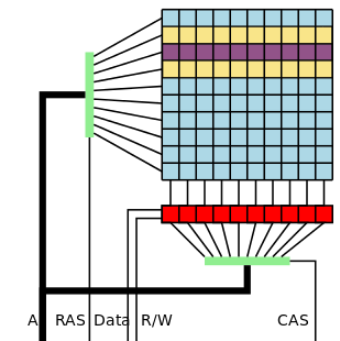
\includegraphics[width=0.45\textwidth]{rowhammer_vis.png}
  \end{center}
  \caption{Rapid row activations (yellow rows) may change the values of bits stored in victim row (purple row).}
\end{figure}
%\begin{wrapfigure}{r}{0.4\textwidth}
%  \begin{center}
%    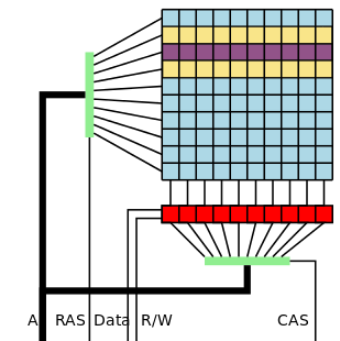
\includegraphics[width=0.3\textwidth]{rowhammer_vis.png}
%  \end{center}
%  \caption{Rapid row activations (yellow rows) may change the values of bits stored in victim row (purple row).}
%\end{wrapfigure}

In 2015, Project Zero, a team of security analysts employed by Google tasked with finding zero-day vulnerabilities, disclosed an attack they named Rowhammer, that would allow for bit flips in a system.
Because newer DRAM has such a high cell density, millions of repeated accesses per second (i.e. hammering) on rows of cells of memory can lead to bit flips in neighboring rows.
A rowhammer attack bypasses memory protection, as one process can affect others, making it very hard to defend against.

%An example of a rowhammer attack is shown in figure \ref{fig:rowhammer_x86} where an attacker repeatedly reads two values, bypassing the cache.
%
%\begin{wrapfigure}{r}{0.4\textwidth}
%  \begin{center}
%    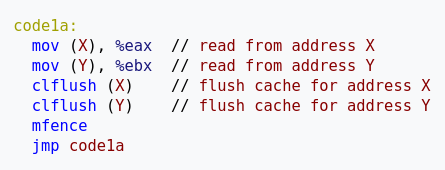
\includegraphics[width=0.4\textwidth]{rowhammer_x86.png}
%  \end{center}
%  \caption[caption]{Small x86-snippet that induces the row hammer effect\hspace{\textwidth} From Blackhat2015 talk [CITE: Blackhat2015\_rowhammer]}
%  \label{fig:rowhammer_x86}
%\end{wrapfigure}

Attacks from the Rowhammer-family, such as Throwhammer, RAMBleed and NetCAT, that perform read/write on memory have since been shown to cause all kinds of havoc from privilege escalation to keylogging to breaking cryptographic keys\cite{tatar_throwhammer:_2018}\cite{kwong2020rambleed}\cite{kurth_netcat:_2020}.
It is worth mentioning, however, that side-channel attacks are highly implementation specific and thus much harder to generalize than if you were to break the algorithm.

\subsubsection{Cold boot attacks}
In 2008, a research paper on cold boot attacks\cite{Halderman2008LestKeys} was published from Princeton University. By physically freezing the memory, attackers were able to read data from the DRAM up to several minutes after cutting power to the victim machine. Cutting power to the victim computer leaves it with no chance to erase its sensitive data from memory. From there an attacker can either restore power and launch a custom kernel leaving a small memory footprint, or transplant the DRAM modules to another computer keeping the DRAM completely intact.

In theory, Hermes is vulnerable to cold boot attacks. In practice, however, it would be near impossible simply because Hermes clears memory after it has run so the power would have to be cut at the exact time where the sensitive data is used. Another property Hermes has, that makes it really difficult to do cold boot attacks is the fact that Hermes uses pass-by-reference. Values are easily corrupted and inline updates are frequent.

\subsubsection{Simple Power Analysis}
Simple Power Analysis (SPA), which is one of two main power consumption analysis methods, focuses on the \emph{operations} that have taken place can tell an attacker a lot about what encryption algorithm is being used.
For example, 10 similar operations in a row can indicate that the algorihtm is AES due to its ten rounds of encryption. 16 rounds could indicate it may be Twofish etc.

This is a very effective method of analysis if the instruction flow depends on the data. 
Modular exponentiation is an example of this: if the square operation is implemented differently than the multiply, (which is a tempting choice since it can be optimized for running time) then the powertrace of an exponentiation directly yields the exponents value.
The following figure shows how SPA has been used to cryptanalyze an RSA algorithm:
\begin{figure}[htp]
  \begin{center}
    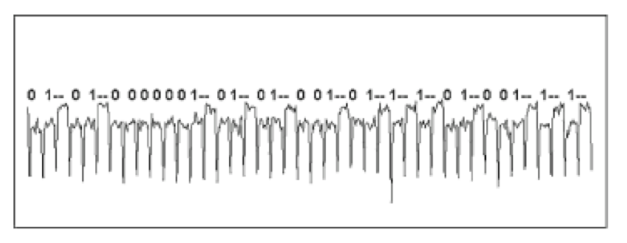
\includegraphics[scale=0.5]{SPA_leaks_from_RSA_implementation.png} \\
  \end{center}
  \caption[caption]{SPA leaks from an RSA implementation. \hspace{\textwidth} From Introduction to Differential Power Analysis \cite{KOCHER2011}}
\end{figure}

%Differential Power Analysis (DPA) takes multiple traces of two sets of data, then computes the difference of the averages. Given enough traces, even tiny correlations can be seen, regardless of how much noise is in the system, since it will effectively cancel out during the averaging.

